\subsection{Total Variation(TV) Based Applications}
\label{subsec:TV Applications}

TV has been a popular tool for image processing tasks, such as denoising, reconstruction, and segmentation\cite{chambolle2010introduction}, the underlying model for TV methods also aims at exploiting the sparsity of the gradient of the image just like the idea of image smoothing\cite{xu2011image} mentioned above. The discrete variant yields the following convex objective function

\small{
\begin{equation}
 \label{eq:descreteTV}
 TV(u)=\sum_{i,j}^{}\|D_{i,j}u\|_2
\end{equation}
}
\\
where $D_{i,j}$ is the discrete gradient operator at pixel $(i,j)$ and $u$ is a vector containing the gray-level pixel values. TV methods filter the image by minimizing $TV(u)$ which is in fact the $l_1$ norm of the vector $[\cdots~\|D_{i,j}u\|_2~\cdots]$.

Since TV is designed for images, it is not directly applicable to geometry processing problem.
As we have stated, the key point is to find some form of second order information.


\subsection{Point cloud consolidation}
\label{subsec:TVPoint cloud consolidation}

Similar to the sparse gradient minimization, and based on the observation that the gradients of smooth surface normals are sparse,
\cite{avron2010L1} formulates their piecewise smoothness reconstruction problem as a sparse minimization of orientation differences and position projections as following

\small{
\begin{equation}
 \label{eq:TVconsolidation1}
 \begin{aligned}
 &N^{out} =\mathop{\argmin}_{N} \sum_{(p_{i},p_{j})\in E}^{} w_{i,j}\|n_{i}-n_{j}\|_2\\
 &s.t.~\forall i~\|n_{i}-{n_{i}}^{in}\|_2\le \gamma_{n}
 \end{aligned}
\end{equation}
}
\small{
\begin{equation}
 \label{eq:TVconsolidation2}
 X^{out} = \mathop{\argmin}_{X} \sum_{(p_{i},p_{j})\in E}^{} w_{i,j}|n_{i,j}\cdot (x_{i}-x_{j})|
\end{equation}
}

Convexity of these two problems allows for finding a global optimum and deriving efficient solvers.
Figure... shows a well reconstructed example with sharp features.
Due to the global nature, this algorithm is extremely slow.
And it may fail for the point set with severe noises and outliers.

\begin{figure}[ht]
  \centering
  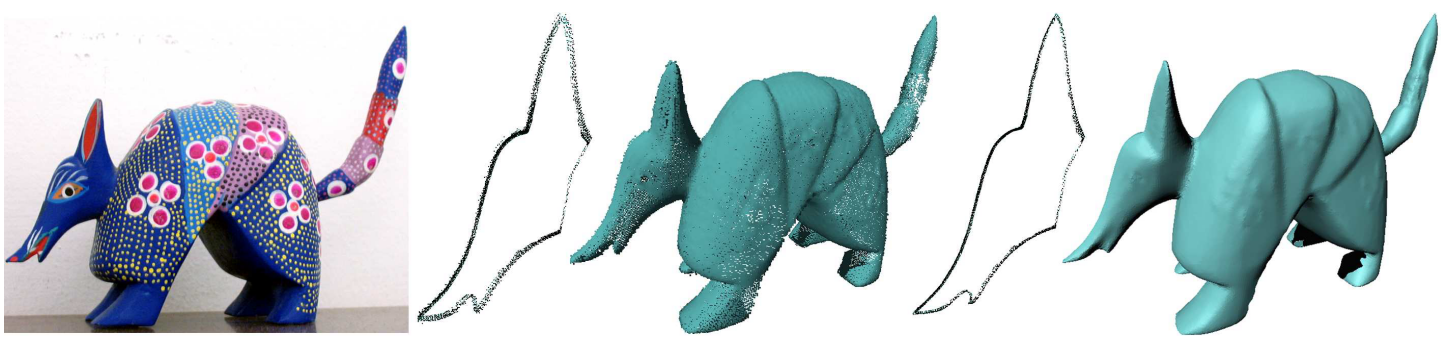
\includegraphics[width=3in]{images/TV_consolidation}
  \caption{Sparse regularization: TV based point cloud consolidation\cite{lipman2007parameterization}. The }
  \label{fig:TV consolidation}
\end{figure}


\subsection{Barycentric coordinates}
\label{subsec:Barycentric coordinates}

Barycentric~coordinates provide a simple and convenient way of interpolating values from a set of control points over the interior of a domain, using weighted combinations of values associated with different control points.

Many barycentric coordinates typically are of global nature, meaning that the interpolated value depends on many, potentially $all$, control points. Besides the lack of locality and scalability, the interpolation is computationally expensive since it involves a weighted sum of all control points for each interior vertex.
Thus, barycentric coordinates with locality provide benefit in terms of storage requirements as well as computational cost.

\cite{zhang2014local} introduces a novel method to derive $local~barycentric~coordinates$(LBC), which depend only on a small number of control points.
Given a set of control points $\mathbf{c}_1, \cdots, \mathbf{c}_n$ in $\mathbb{R}^2$ or  $\mathbb{R}^3$ which are the vertices of a closed control cage, and let the domain bounded by the cage.
They want to find a function $w_{i}$: $\Omega\rightarrow\mathbb{R}$ for each $\mathbf{c}_{i}$, such that $[w_1(\mathbf{x}), \cdots, w_n(\mathbf{x})]$ is a set of generalized barycentric coordinates of $\mathbf{x}\in\Omega$ with respect to the control points $\{\mathbf{c}_{i}\}$ and is used for interpolating function values $f(\mathbf{c}_1), \cdots, f(\mathbf{c}_n)$ at control points on the interior of $\Omega$ by

\small{
\begin{equation}
 \label{eq:BC}
 f(\mathbf{x}) = \sum_{i=1}^{n}w_{i}(\mathbf{x})f(\mathbf{c}_{i})
\end{equation}
}
\\
here, except for the properties satisfied in many barycentric coordinate schemes, like reproduction, partition of unity and non-negativity, they prefer a target functional that reflects locality and smoothness for the coordinate functions while still convex.

For a function $w_{i}$ and a given value $s$, denote by $\{w_{i}>s\}:=\{\mathbf{x}|w_{i}(\mathbf{x})>s\}$ and $\{w_{i}=s\}:=\{\mathbf{x}|w_{i}(\mathbf{x})=s\}$ the $superlevel~set$ and the $level set$ of $s$, respectively.
Locality requires the area of the superlevel set $\{w_{i}>0\}$ to be small which means that the vector$[w_{1}(\mathbf{x}), \cdots, w_{n}(\mathbf{x})]$ is sparse, while for smoothness it is necessary that all curves/surfaces $w_{i}=\textrm{const}$ are smooth.

Based on these observations, the locality and smoothness of $w_{i}$ can be obtained using a functional that measures the sum of the sum of the perimeters of superlevel sets $\{w_{i}>s\}$ for all $s$.
And then the perimeter of each superlevel set regularizes the smoothness of its boundary level curve/surface, while the perimeter of $\{w_{i}>0\}$ penalizes the area of the influence region. It turns out that this functional is exactly the total variation of $\{w_{i}\}$. Finally, the problem is formulated as

\small{
\begin{equation}
 \label{eq:LBC}
 \begin{aligned}
 & \min_{w_1, \cdots, w_2} \sum_{i=1}^{n} \int_{\Omega}^{} |\bigtriangledown w_{i}| \\
 & ~~~s.t.~ \sum_{i=1}^{n}w_{i}(\mathbf{x})\mathbf{c}_{i}=\mathbf{x},
        \sum_{i=1}^{n}w_{i}=1,~w_{i}\geq0,~\forall \mathbf{x}\in\Omega,\\
 & ~~~~~~~~w_{i}(\mathbf{c}_{j})=\delta_{ij},~forall i,j,\\
 & ~~~~~~~~w_{i}~\textrm{is linear on cage edges and faces }\forall i.
 \end{aligned}
\end{equation}
}

Figure~\ref{fig:LBC} shows a cage-based deformation example with lower computational and storage requirement since each point on the target shape is only determined by a small number of control points.
Whatever, from the observation, we can see that there is a trade-off between locality and smoothness which is a common troubling issue for so many existing works.

\begin{figure}[ht]
  \centering
  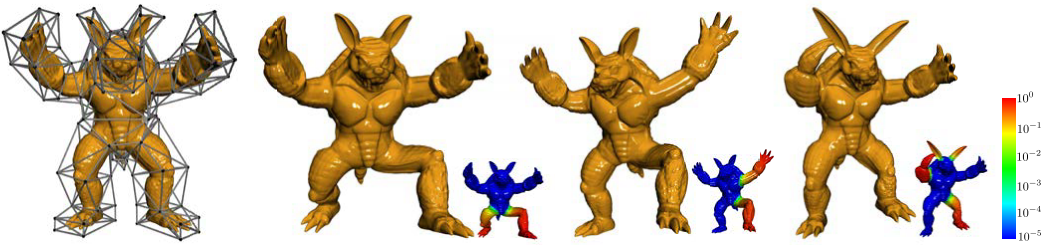
\includegraphics[width=3in]{images/LBC_L1}
  \caption{Sparse regularization: TV based local barycentric coordinates\cite{zhang2014local}. Using LBC for 3D cage-based manipulation allows for local, smooth and shape-aware deformations. Only parts near the manipulated control points are deformed, as indicated by the color-coding.}
  \label{fig:LBC}
\end{figure}
